\section{Overview}
  \paragraph\
    In this chapter I describe about \emph{ntop}, Cassandra and the implementation of Cassandra plugin for \emph{ntop}. I also specify the design and implementation of Cassandra client for C that was developed using C-python API. 
% I have done few testing of my solution that I describe in results section.

\section{\emph{ntop}}
  \emph{ntop} is an open-source traffic measurement application written in C. \emph{ntop} design follows the UNIX philosophy: applications can be divided into small independent pieces that co-operate to achieve a common goal.
  \emph{ntop} has the following modules:
%AP: Case of the Missing Articles - I can write a nice long story about missing articles ``a, an, the'' in students' reports I think! Also, it seems not to matter how many times I talk about the singular and plural noun and verb combinations! I have to correct almost every sentence for this error. When will you guys ever learn?!
    \begin{enumerate}
     \item Packet Sniffer - Capture packets using \emph{libpcap} library and also from UNIX sockets.
     \item Packet Analyzer - Analyze packets captured by Packet Sniffer.
     \item Traffic Rules - \emph{ntop} allows traffic rules for capturing packets to filter out unnecessary packets.
     \item Report Engine - Report Engine displays analyzed output in an interactive web-based user interface. 
     \item Plugins - Using plugins anyone can extend \emph{ntop} to support extra features.
    \end{enumerate}

\subsection{Packet Sniffer}
\paragraph\
	Packet Sniffer captures packets using \emph{libpcap} library and stores them into internal buffer. This helps reduce packet drops	in a busty traffic environment. \emph{libpcap} is supported by all major Operating Systems, that allows \emph{ntop} to be portable to Windows and UNIX variants.

        \begin{figure}[htb]
          \centering
          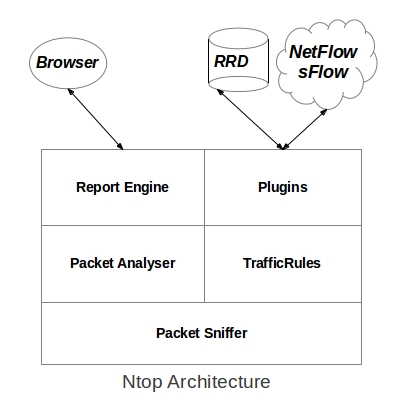
\includegraphics[scale=.5]{ntoparc.jpg}
          \caption{Architecture of \emph{ntop}.} 
        \end{figure}

	\subsection{Packet Analyzer}
	 \paragraph\
	 Packet Analyzer gets packets from Packet Sniffer and processes those packets. Sniffed packets contains information about status of the network and that information is calculated by Packet Analyzer and then stored in 
	 RRD for future references.

	\subsection{Traffic Rules}
	\paragraph\
	  \emph{ntop} allows user to specify what kind traffic a user is interested in. Using \emph{libpcap} filter expression 
	  \emph{ntop} achieves this goal. Traffic Rules help \emph{ntop} to reduce some burden on memory as well CPU, make \emph{ntop} faster as it processes less number of packets.

	\subsection{Report Engine}
	\paragraph\
	  \emph{ntop} contains a web server by which users from any geological location can monitor their network.
	  Report Engine provides a beautiful user interface with time series graph drawn using RRDTool. Using Report Engine
	  a user can change the behavior of \emph{ntop} by changing its configuration parameters.

	\subsection{Plugins}
	 \paragraph\
	 \emph{ntop} has flexible design that allows user to add their own plugins. At startup \emph{ntop}
	 searches shared libraries (like .so, .dll files) to load  plugins. A plugin can access \emph{ntop}'s global 
	 data structure and can use API exported by \emph{ntop}.

\section{Cassandra Database}
\paragraph\
      Cassandra is a highly scalable and highly available database initially developed by Facebook using two famous approaches: GFS \cite{gfs} from Google and Dynamo \cite{dynamo} from Amazon. Cassandra is highly used in ebay and Netflix. 

      Cassandra's big data features are \cite{}
      \begin{enumerate}
       \item Elastic scalability.
       \item High availability.
       \item Distributed database design with no single point of failure.
       \item Blistering linear performance.
       \item Multiple datacenter based data distribution.
      \end{enumerate}
      %new items after Ma'am first review
      \subsection{Cassandra Architecture:}
      \paragraph\
	  Cassandra has a peer-to-peer distribution model. Therefore all nodes in a Cassandra cluster are symmetric.
	  Any node can take read/write requests from clients and forwards them to correct node on the cluster. This design makes 
	  Cassandra scalable. Cassandra uses Gossip \cite{gossip} protocol for intra-ring communication to support decentralization and partition 
	  tolerance. Gossip protocol helps to detect failures and recovery Cassandra node as well.
	      \begin{figure}[htb]
		\centering
		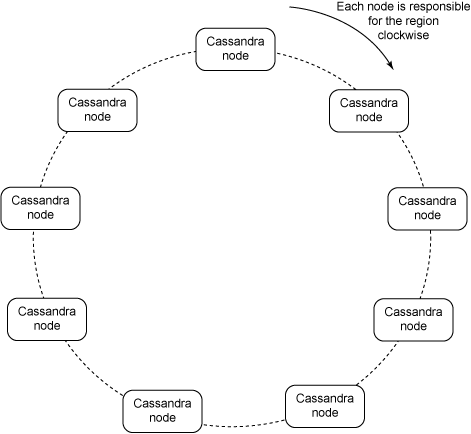
\includegraphics[scale=.5]{cassandra_ring.png}
		\caption{Cassandra Ring \cite{cassandra_ring}} 
		\label{Cassandra_ring}
	      \end{figure}
	 Figure \ref{Cassandra_ring} describe about Cassandra ring.
	 \paragraph{Cassandra Data Model:}
	  Cassandra uses dynamic schema, column oriented data model. A database in a Cassandra named by keyspace consists of column families.
	  A column family is a group of key-value pairs sorted by column name. A node in Cassandra cluster gets a token range at start up and also gets 
	  ownership of all keys that fall into the token range. Keys in a column families sorted according to the partition
	  of the Cassandra cluster. There are two partitioning  scheme for a Cassandra cluster.
	  \begin{enumerate}
	   \item  Random Partitioner: It uses 128 bit MD5 hash value of key to get a token. It is default partitioning strategy that helps 
		  automatic load balancing as md5 hash value ensure key distribution.
	   \item Ordered Partitioner: It uses byte order of key as token. It allows range scans over rows.
	  \end{enumerate}
	  Figure \ref{cassandra_data_model} describes Cassandra data model.\\
	      \begin{figure}[htb]
		\centering
		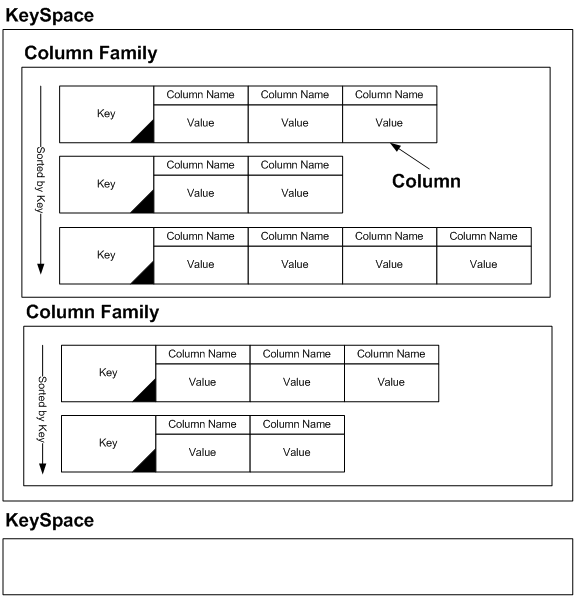
\includegraphics[scale=.5]{cassandra_data_model.png}
		\caption{Cassandra Data Model} 
		\label{cassandra_data_model}
	      \end{figure}
	  Below table compares RDBMS schema with Cassandra data model.\\
	  \begin{table}[ht]
	  \centering
	   \begin{tabular}{|l|l|}
	   \hline
	   {\bf RDMS}     & {\bf Cassandra}      \\ \hline 
	   Database & Keyspace       \\
	   Table    & Column Falily  \\
	   Entity   & Column Name    \\
	   Value    & Column Value   \\ \hline
	  \end{tabular}
	  \caption{Comparison between RDMS schema with Cassandra Data Model}
	  \end{table}
	 \paragraph{Memtables, SSTables and commit log:}
	    Cassandra uses in-memory data structures called memtable for caching recent writes to a Cassandra node.
	    Memtables are later stored into disk as SSTables depending on timeout or  memtable threshold size. In a write operation
	    a Cassandra node first writes into commit log then to memtable. Data recovery is done by commit log. In case of reading 
	    Cassandra maintains row cache key cache to make read operation faster. Figure \ref{cassandra_rw} describes read/write
	    operations in a Cassandra node.
	      \begin{figure}[htb]
		\centering
		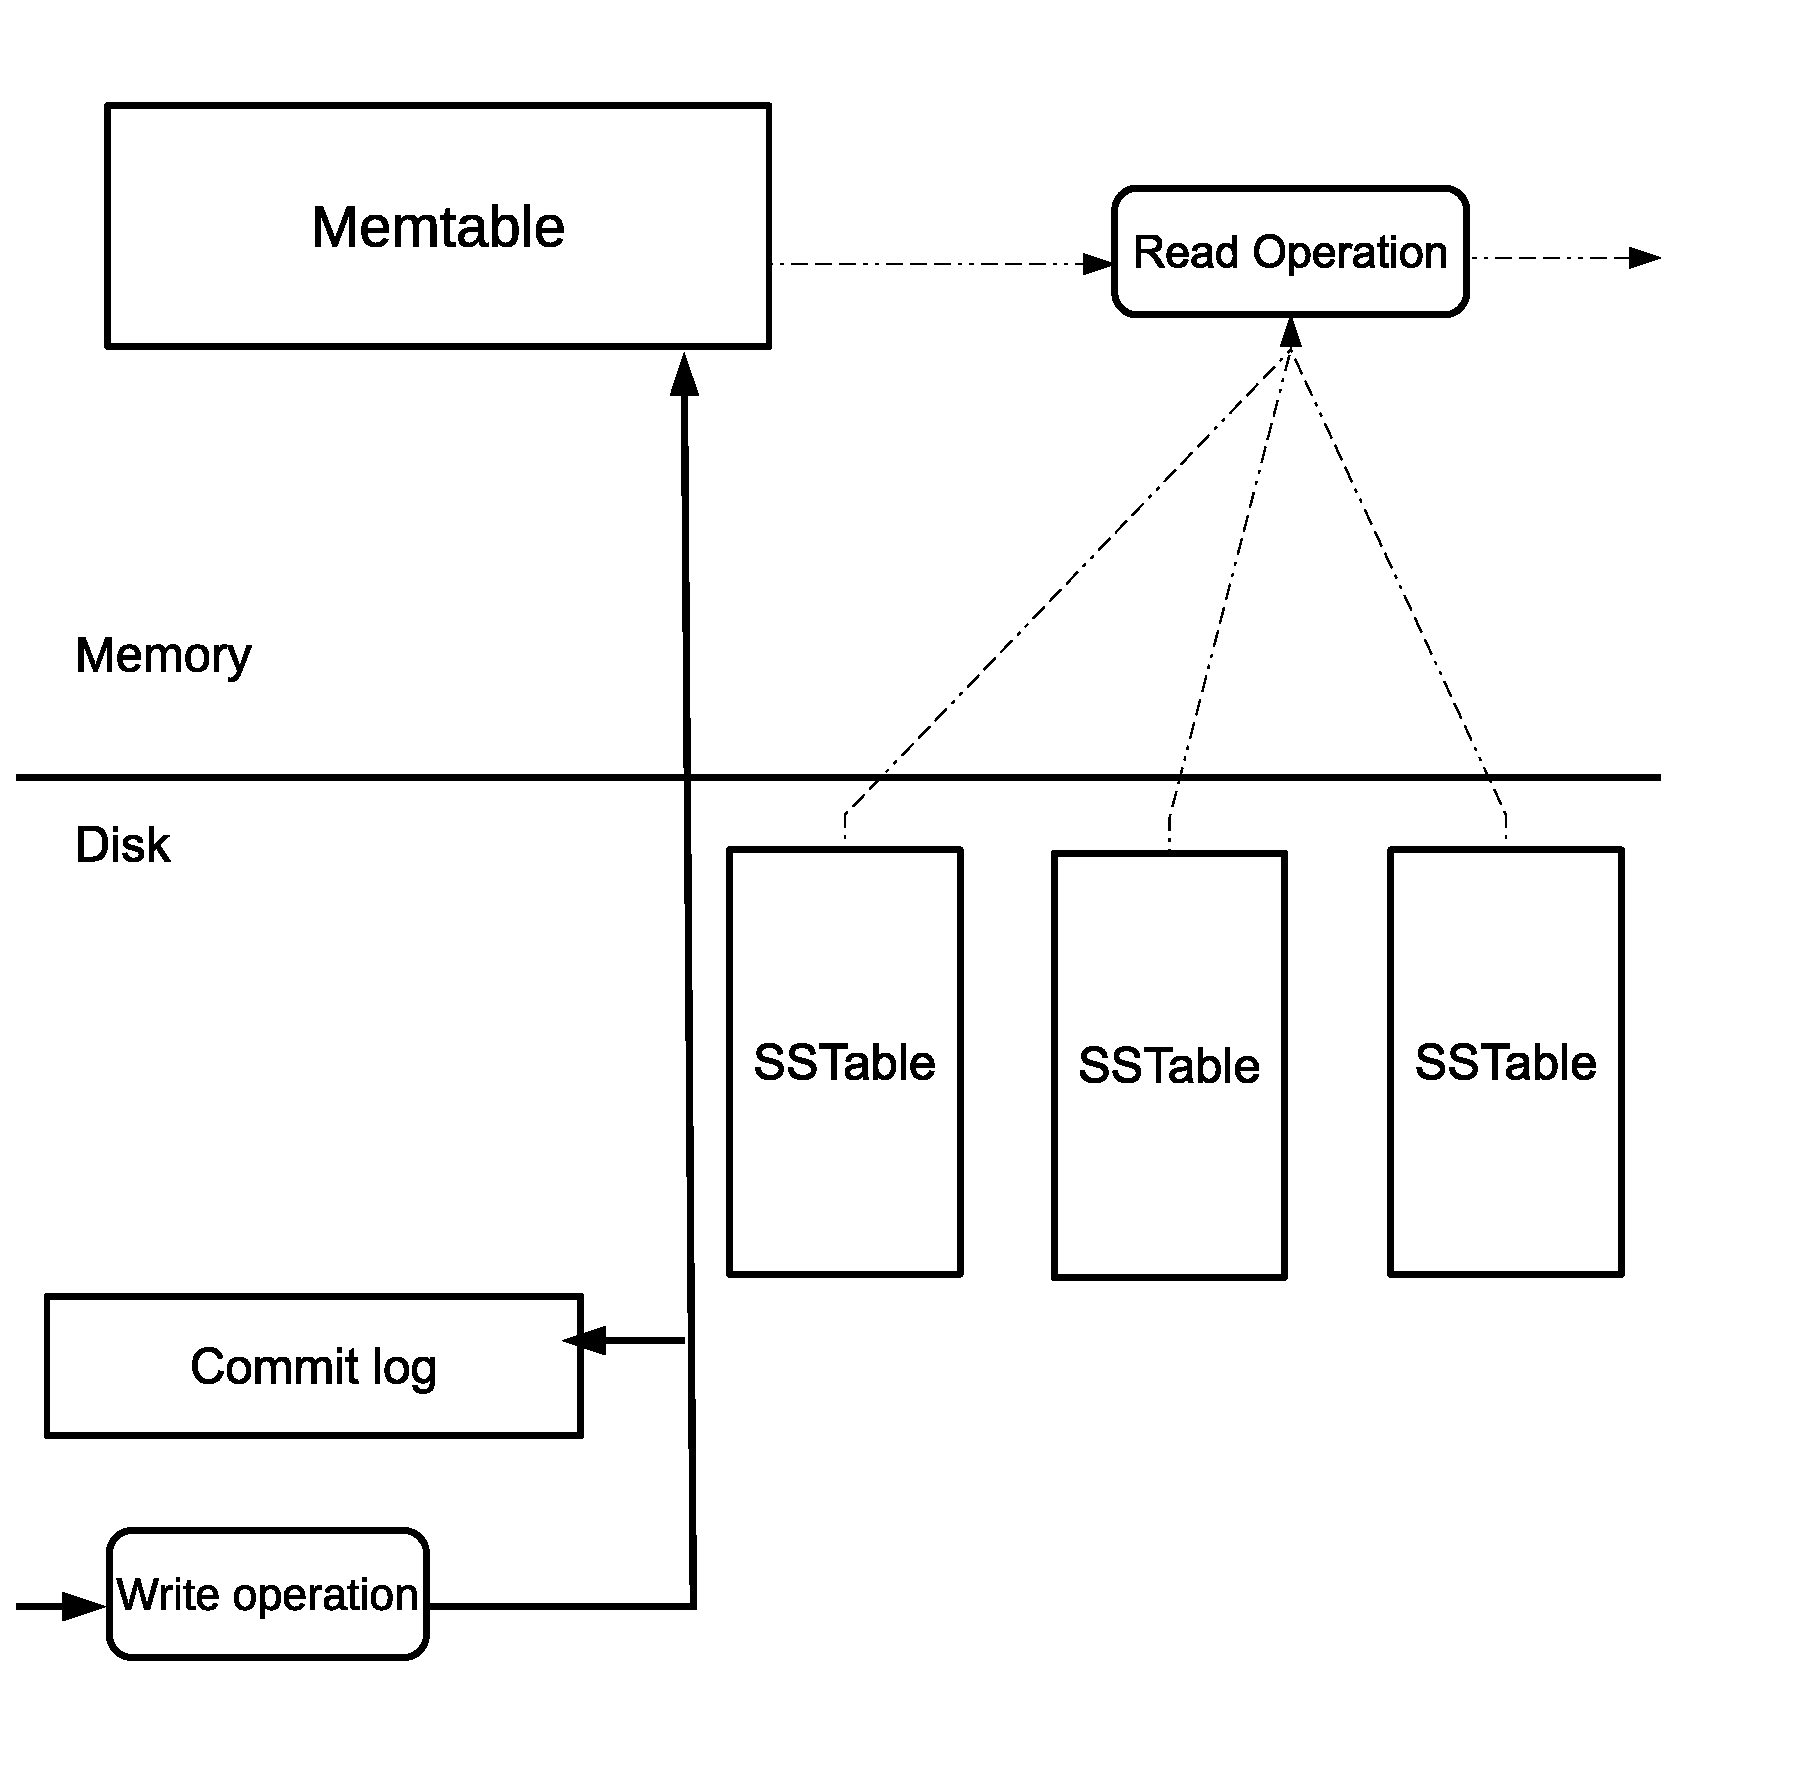
\includegraphics[scale=.35]{cassandra_rw}
		\caption{Cassandra Read/Write operation} 
		\label{cassandra_rw}
	      \end{figure}

	    %new items after Ma'am first review
      \subsection{Why Cassandra}
      \paragraph\
	  In one of our testbeds we are able to generate approximately 1000 NetFlow packets per second with only two nodes
	  having 1 Gbps NIC card. The table \ref{datagenerated} provides the amount of data generated by our testbed.
	  
	  \begin{table}[ht]
	  \centering
	  \label{datagenerated}
	    \begin{tabular}{ccc}
	      \\
	      \hline
	      Packets generated& Time & Size of generated data \\
	      \hline
	      1000   & 1 second & 1.4MB\\
	      60 k   & 1 minute & 85 MB\\
	      3.6 m  & 1 hour    &  5 GB\\
	    \end{tabular}
	    \caption{Data generated by two node testbed.}
	    \label{datagenerated}
	   \end{table}
	  
	It is clear that we cannot use RDMS based databases for storing flows in data center networks as they create explosive amount of data in a short time. 

	The features required of a database for flow monitoring are:
	\begin{enumerate}
	  \item Scalability : so that huge amount of data can be stored according to the demand.
	  \item High write throughput : As flow records are generated at a rapid pace in data center networks, a flow monitoring system needs to write them fast.
	  \item Reasonable read performance : For real-time flow processing.
	  \item MapReduce support: For offline flow processing it needs to support MapReduce to enable massive data crunching operation.
	\end{enumerate}

	\paragraph{Redis:} Redis is written in C. It has fast read-write performance but is not scalable. Redis cluster, which is expected to support scalability, is going to be launched by the end of 2013 \cite{rrdcluster}. 
	\paragraph{HBase:} HBase is written in Java. It is scalable, has good read/write performance but is suitable only for batch processing. It has a single point of failure with Hadoop NameNode due to which HBase may lose data.
%for which HBase may lose data  .  

	\paragraph{Cassandra:} Cassandra meets all the requirements that are needed.
          \begin{figure}[htb]
	    \centering
	    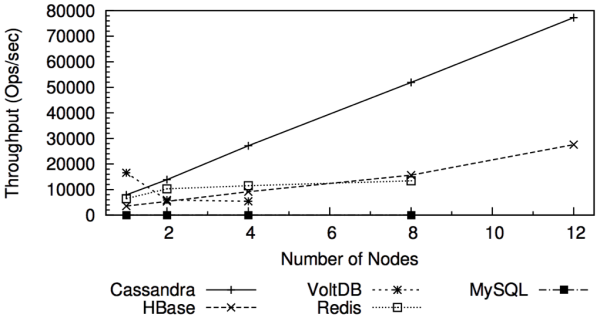
\includegraphics[scale=.5]{cassathpt.png}
	    \caption{Cassandra Performance \cite{cassathpt}.} 
	  \end{figure}

\section{Cassandra C Client}
\paragraph\
      Cassandra C client is a wrapper developed by me around Cassandra Python client, $Pycassa$. This allows any user to call Cassandra API from a C program.
%I used C-Python API to write wrapper around Python's Pycassa API. 
Pycassa uses Thrift RPC call to communicate with Cassandra. Fig. \ref{cass-c-api} shows the architecture of the Cassandra C API.
      
%Figure 2.3 describes how a C client API call finally reach Cassandra. 
Cassandra C client API has three major classes of APIs. These are 
      \begin{enumerate}
       \item Schema Manipulation API: Manages schema definitions of Cassandra.
       \item Data Manipulation API: Inserts or retrieves data from Cassandra. 
       \item Utility API:  API that do some common useful work. 
      \end{enumerate}

      \begin{figure}[htb]
	 \centering
         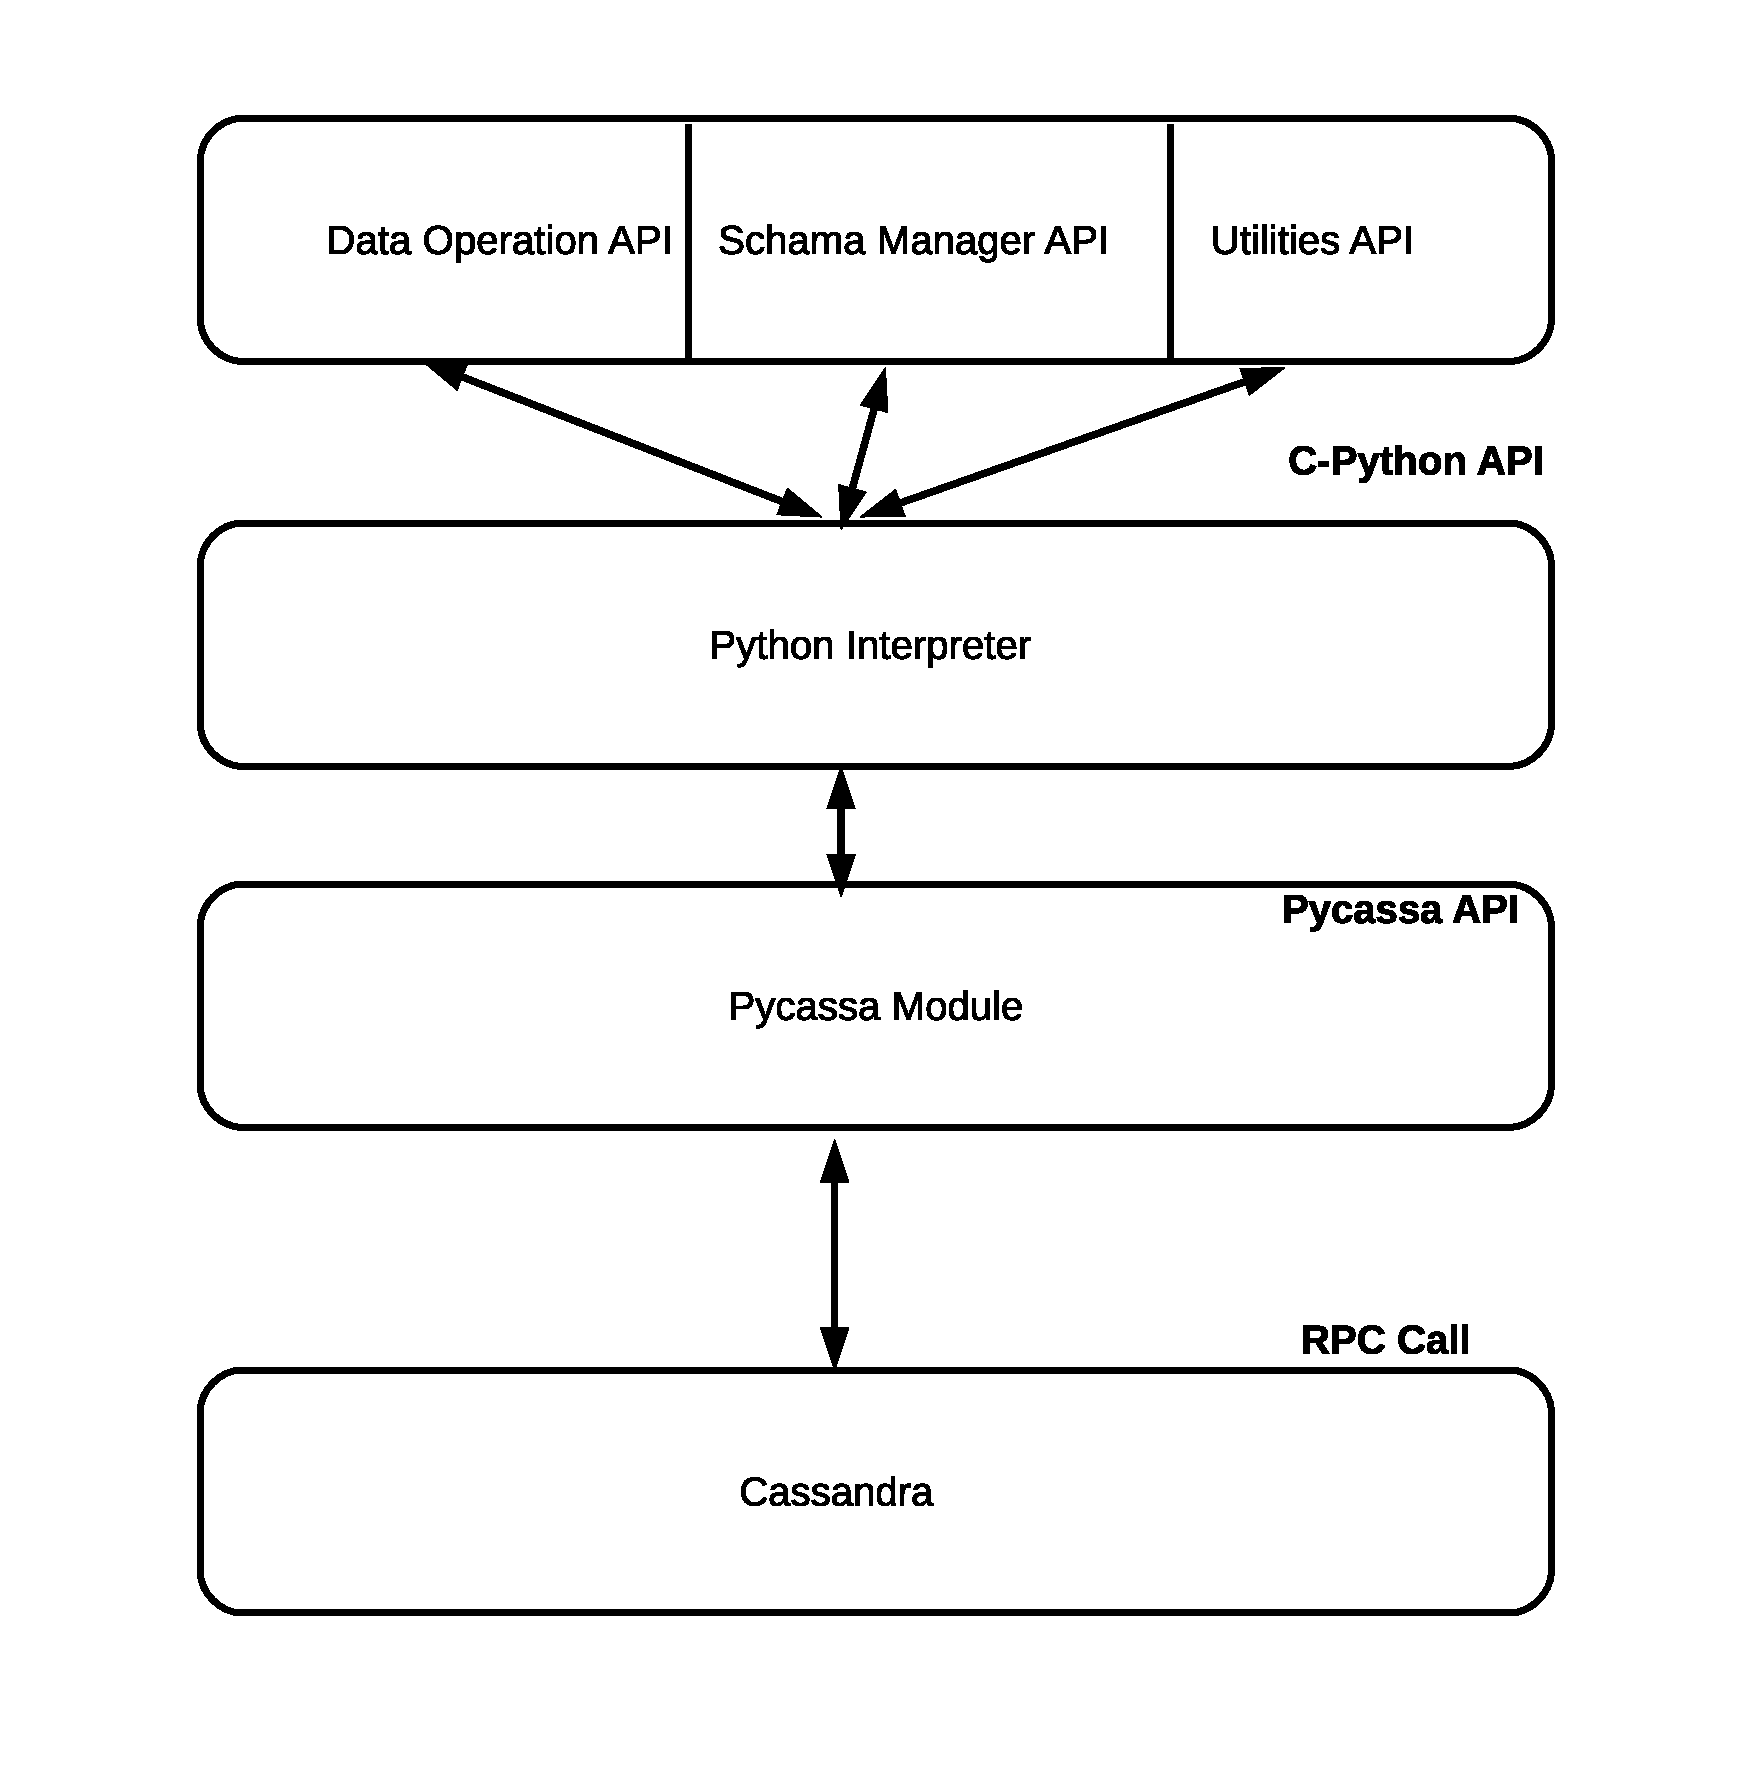
\includegraphics[scale=0.3]{C_client}
         \caption{API interaction with Cassandra }
	\label{cass-c-api}
      \end{figure}

\subsection{Schema Manipulation API}
      \paragraph\
      These APIs allow one to create or delete keyspace and column families. 

      \begin{enumerate}
       \item {\bf cassandraCreateKeyspace}(name, server, rf, strategy): Create a keyspace on the server with the given replication factor(rf) and strategy.
	    Supported strategies are :
	     \begin{enumerate}
	      \item SimpleStrategy : Replication strategy that simply chooses consecutive nodes in the ring for replicas.
	      \item NetworkTopologyStrategy : Replication strategy that puts a number of replicas in each data center.
	      \item OldNetworkTopologyStrategy : OldNetworkTopologyStrategy is provided for backwards compatibility with old Cassandra installations.  %AP re-write this.
	     \end{enumerate}

       \item {\bf cassandraCreateColumnFamily}(name, keyspace, comparator, server): Create a column family on the keyspace with the given comparator. 
	      Supported comparators are :
		    \begin{enumerate}
		     \item AsciiType
		     \item DoubleType
		     \item IntegerType
		     \item BytesType
		     \item LongType
		     \item FloatType
		     \item TimeUUIDType
		    \end{enumerate}

      \item {\bf cassandraDropColumnFamily}(name, keyspace, server): Delete the given column family, $name$, from the keyspace.

      \item {\bf cassandraDropKeyspace}(name, server): Delete keyspace, $name$, from the server.
      \end{enumerate}

    \subsection{Data Manipulation API}
    \paragraph\
    These APIs deal with insertion and retrieval of data from the Cassandra server.

      \begin{enumerate}
       \item {\bf cassandraConnect}(keyspace, columnfamily, server): Create a connection and store the connection object in the internal Python dictionary for later use. As connection creation takes time, connection objects are cached in the Python dictionary.

       \item {\bf cassandraInsert}(id, key, value, column name): Insert a key-value pair in the column family referred by $id$.
       \item {\bf cassandraTimeSeriesInsert}(keyspace, cf, server, key, column\_name, value, bkt\_size): cassandraTimeSeriesInsert is a simplified way of inserting time series data into Cassandra with predefine data model. It takes all required arguments and performs the write operation. The argument $bkt\_size$ specifies size of the bucket. A Python dictionary maintains most recent connection objects to make write fast. Figure \ref{datamodel} describes about the data model.

       \item {\bf cassandraGet}(id, key): Return a dictionary of key-value pairs from  the column family referred by $id$.

       \item {\bf cassandraGetItem}(dictionary, position, name, value): Return $name$ and $value$ from given $position$ of the $dictionary$.  %AP: rewrite
      \end{enumerate}

    \subsection{Utility API}
    \paragraph\
    These APIs provide general functionality that we need.

      \begin{enumerate}
       \item {\bf isExistPycassa}(): Check existence of pycassa on the system.
       \item {\bf isExistKeyspace}(name, server): Check existence of keyspace on the server.
       \item {\bf isExistColumnfamily}(name, keyspace, server): Check existence of columnfamily, $name$, on the $keyspace$. 
      \end{enumerate}

      \section{Cassandra Plugin for \emph{ntop}}
      \paragraph\
      Cassandra Plugin is developed in C as a shared object. \emph{ntop} uses  shared objects principles to provide plugins, 
      that allows dynamic linking of compiled shared objects  to \emph{ntop} to add extra features.

      \textbf{The APIs supported by \emph{ntop} for plugin support are given below:}\\
      \begin{table}[ht]
	\centering
	
	\label{ntopplugin}
	\begin{tabular}{|l|l|}
	    \hline
	    \textbf{API name} &  \textbf{Details}\\
	    \hline
	    int(*IntFunct)(void); & Called at initialization of the plugin.\\
	    \hline
	    void(*VoidFunct)(u\_char); & Called at termination of the plugin.\\
	    \hline
	    void(*PluginHTTPFunct)(char* url); & HTTP request handler function.\\
	    \hline
	  \end{tabular}
	  \caption{APIs for Plugin Support}
      \end{table}      

      \paragraph{API of Cassandra Plugin:} Given below are the APIs developed by me for a
      Cassandra Plugin for \emph{ntop}.\\
      
      \begin{enumerate}
       \item {\bf initCassandraFunct } (void): Initialize Cassandra Plugin. It checks for pycassa module, availability of the Cassandra server and then invokes cassandraMainLoop.
       \item {\bf termCassandraFunct} (u\_char termNtop): Terminates Cassandra Plugin.
       \item {\bf handlecassandraHTTPrequest} (char *\_url): It gets a web request from the web browser and serves them.\\
       \item {\bf cassandraMainLoop}(void) : This API does all major work described below:
	      \begin{enumerate}
	      \item Reads configuration files and initializes the data structure needed to store data.
	       \item Identifies sniffed interface, gets statistics from global variables and stores into Cassandra.
	       \item Identifies NetFlow socket, gets data from global variables and stores them to Cassandra. 
	      \end{enumerate}
      \end{enumerate}

      \subsection{Architecture}
      Figure 2.4 shows the architecture for Cassandra Plugin. \\
           \begin{figure}[htb]
	    \centering
	    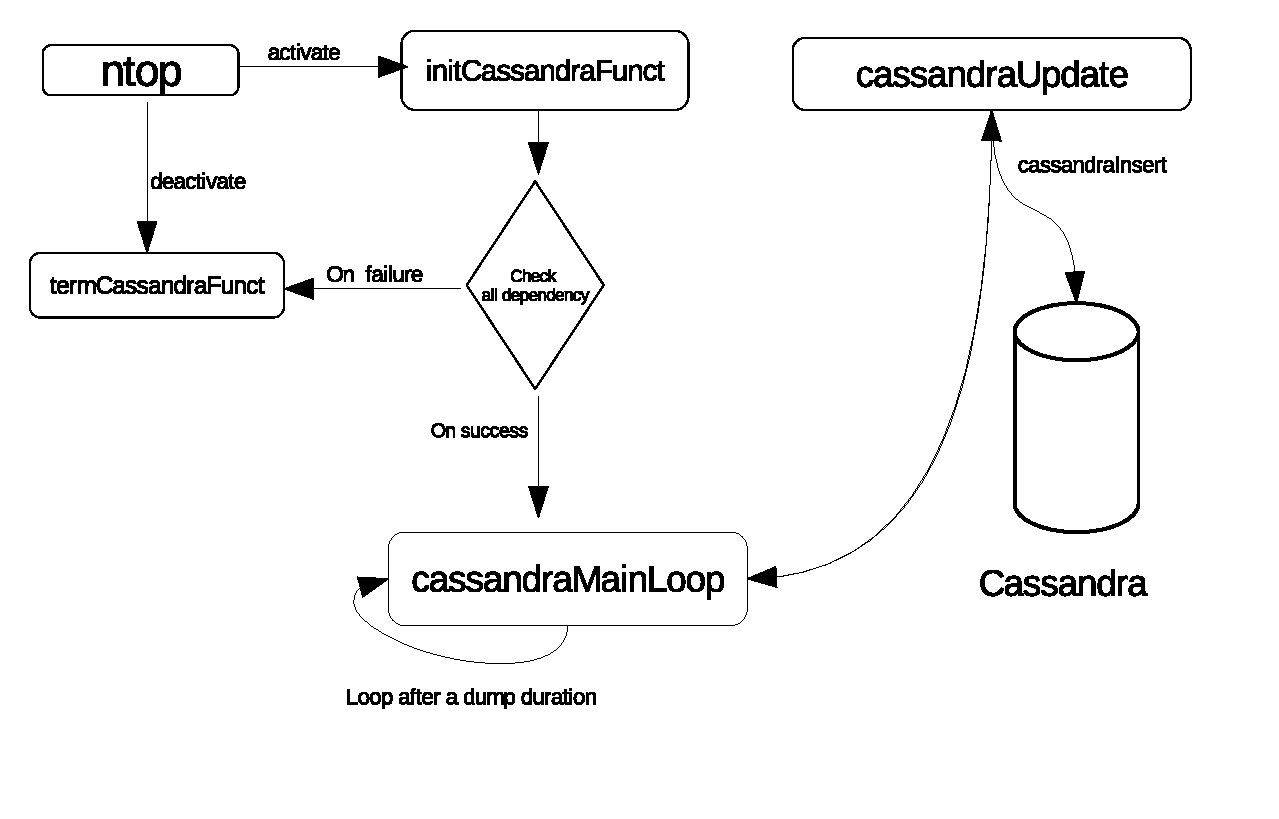
\includegraphics[scale = .7]{lfc}
	    \caption{Architecture of Cassandra Plugin.} 
	  \end{figure}
      Cassandra Plugin for \emph{ntop} stores all statistics in a Cassandra keyspace using cassandraTimeSeriesInsert() API.
      Figure \ref{datamodel} shows the data model used by cassandraTimeSeriesInsert() API. TimeUUIDType is data type for
      a key in Index column family. Unix timestamp is not useful when time series data events occurs at same time. TimeUUIDType is 
      a unique value even for the events that generated at the same timestamp. This plugin going to take dump interval, bucket size for
      cassandraTimeSeriesInsert(), keyspace prefix from a configuration file. There will be one keyspace for every instance of \emph{ntop}.
      Keyspace prefix helps to resolve any collusion. It is preferable to use uuid as keyspace prefix. \emph{ntop} has multiple counters
      for every interface that it monitors. Counters belong to a interface stored into column family created with the name of the interface.
      \begin{figure}[htb]
	    \centering
	    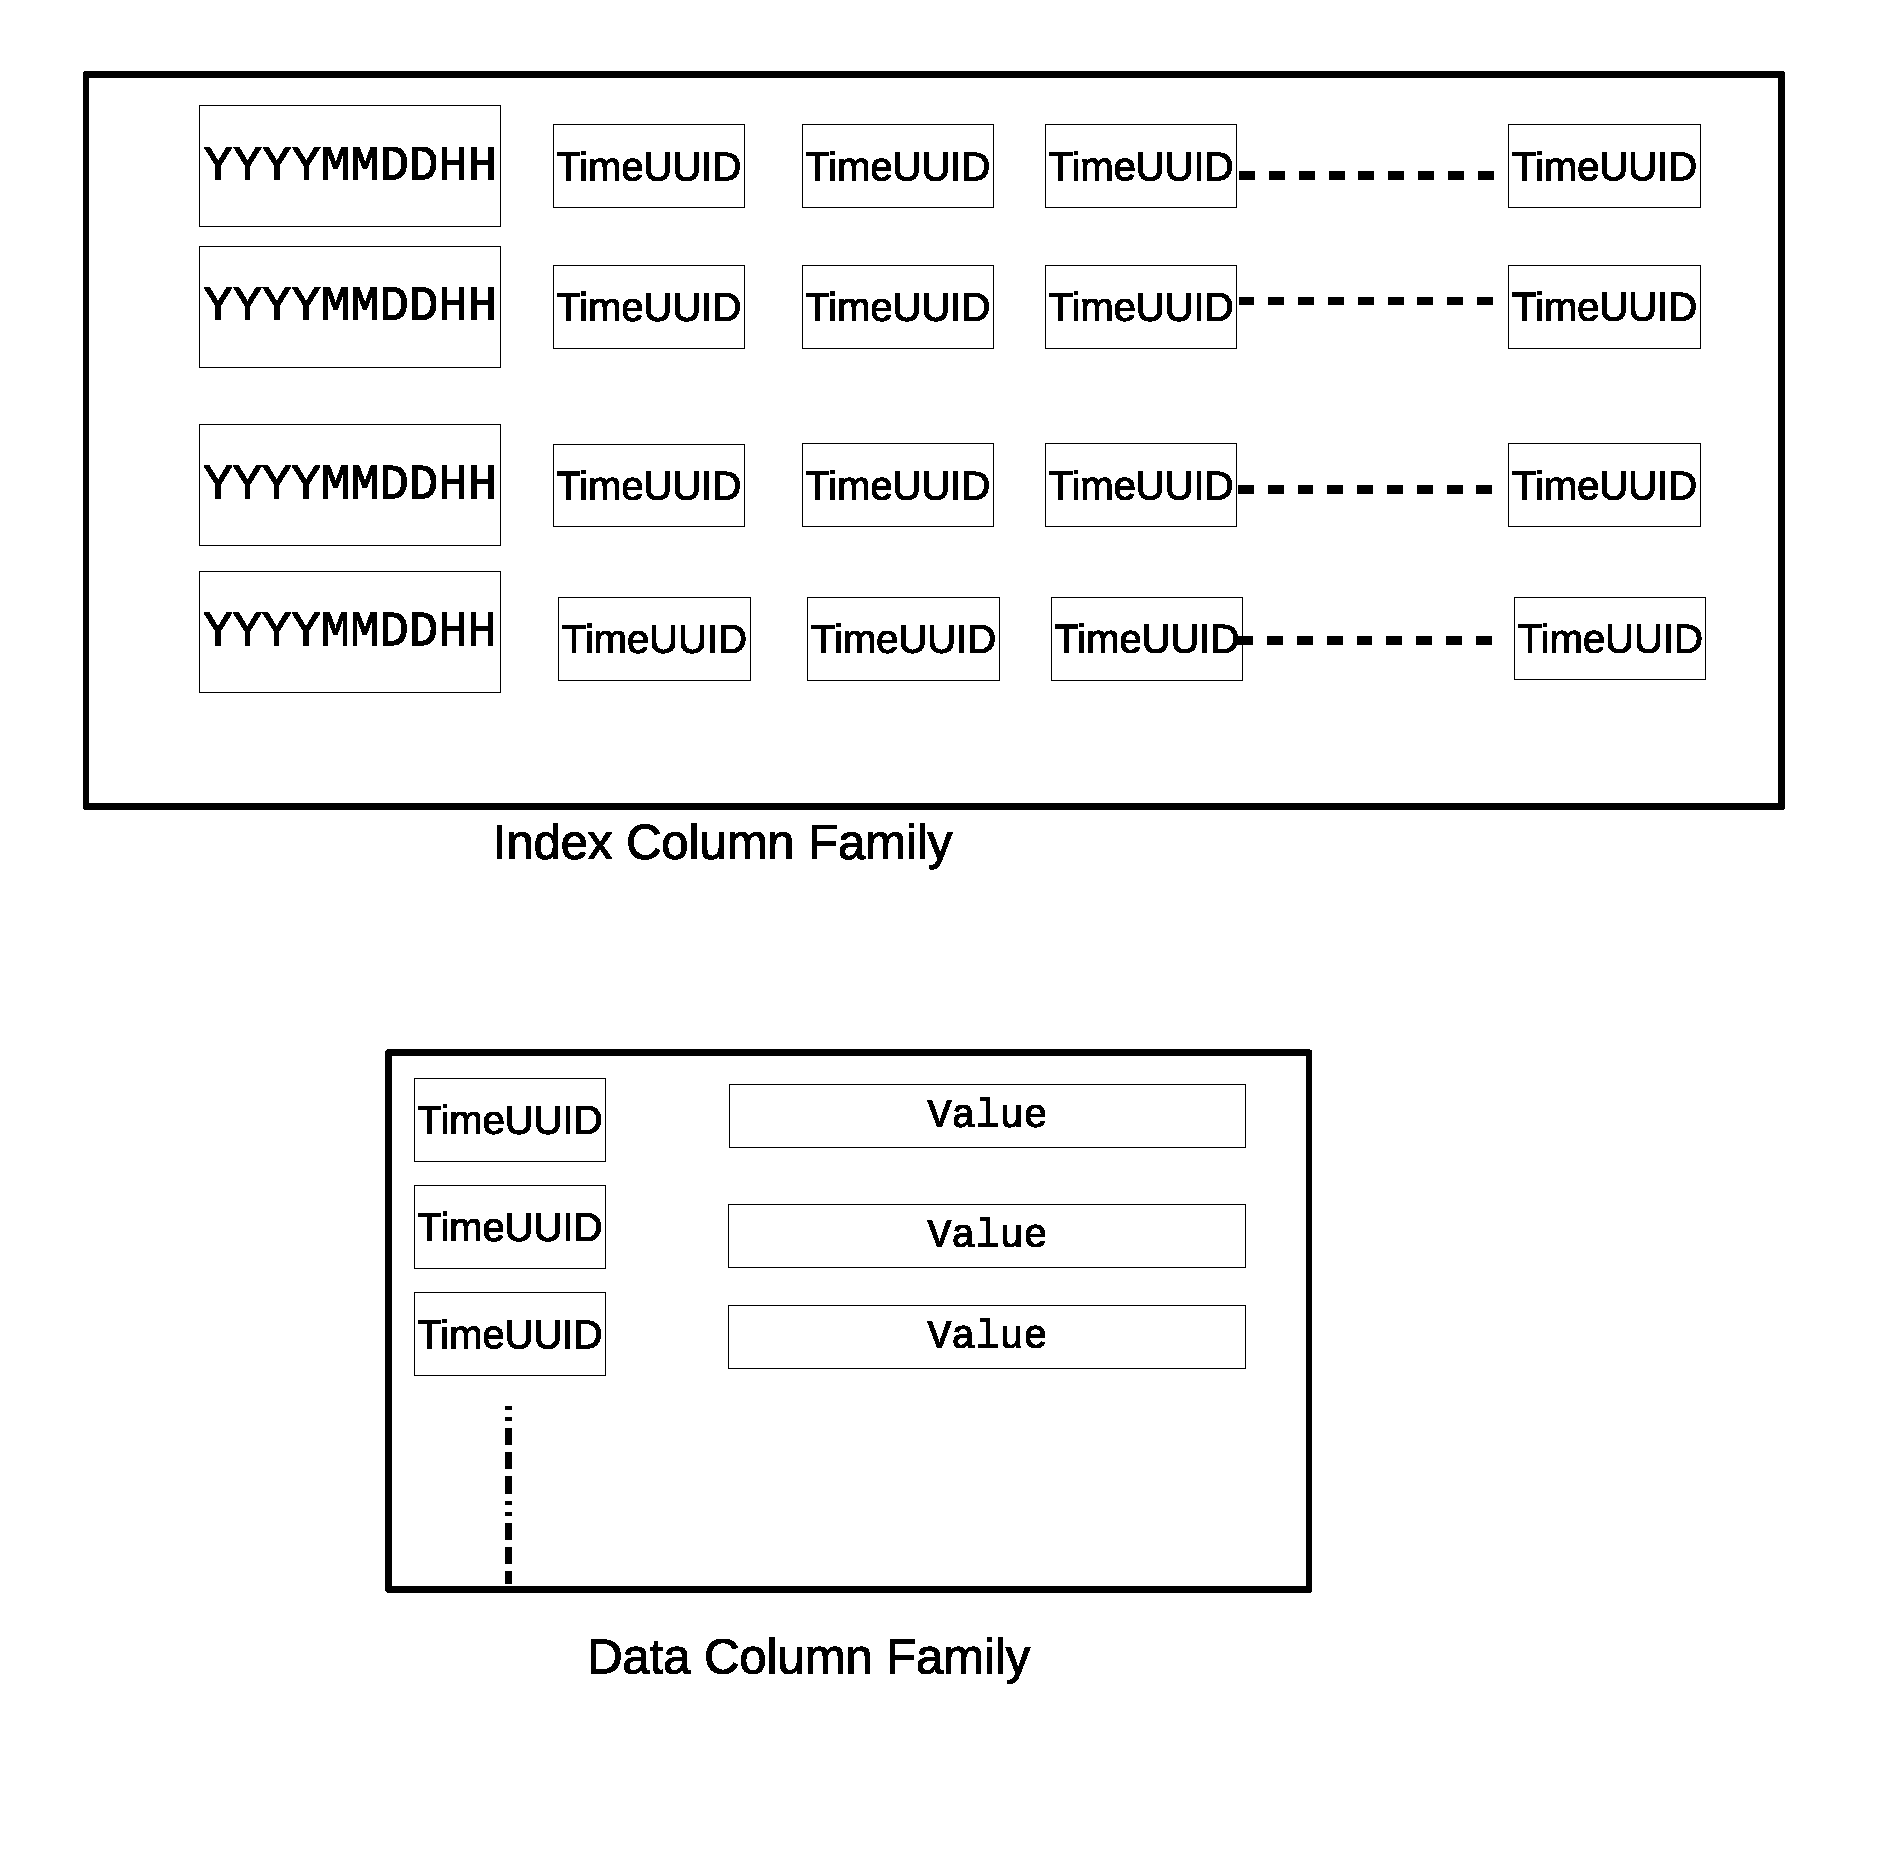
\includegraphics[scale = .4]{data_model}
	    \caption{Data Model for Cassandra \emph{ntop} Plugin.} 
	    \label{datamodel}
	  \end{figure}
	  
      We have tested our Cassandra Plugin \emph{ntop} as well \emph{ntop} running without our plugins. We are sharing the results in the next 
      section.
      \section{Results}
      %TODO
      